\documentclass[conference]{IEEEtran}
\usepackage{cite}
\usepackage{amsmath,amssymb,amsfonts}
\usepackage{algorithmic}
\usepackage{graphicx}
\usepackage{textcomp}
\usepackage{xcolor}
\usepackage{verbatim}
\usepackage{subcaption}
\usepackage{caption}
\usepackage{gensymb}
\usepackage{hyperref}
\def\BibTeX{{\rm B\kern-.05em{\sc i\kern-.025em b}\kern-.08em
    T\kern-.1667em\lower.7ex\hbox{E}\kern-.125emX}}

% commands for fixing the author name centering    
\makeatletter % changes the catcode of @ to 11
\newcommand{\linebreakand}{%
  \end{@IEEEauthorhalign}
  \hfill\mbox{}\par
  \mbox{}\hfill\begin{@IEEEauthorhalign}
}
\makeatother % changes the catcode of @ back to 12

\newcommand{\state}[2]{\boldsymbol{s}^{#1}_{#2}}
\newcommand{\ctrl}[2]{\boldsymbol{u}^{#1}_{#2}}

\newcommand{\radius}[1]{r_{#1}}
\newcommand{\headangle}[1]{\phi_{#1}}
\newcommand{\pos}[1]{p_{#1}}
\newcommand{\vel}[1]{v_{#1}}
\newcommand{\posvec}[1]{\boldsymbol{\pos{}}_{#1}}
\newcommand{\velvec}[1]{\boldsymbol{\vel{}}_{#1}}

\newcommand{\policy}[1]{\pi_{#1}}
\newcommand{\dt}{\Delta t}

\newcommand{\Reward}[1]{R_{#1}}
\newcommand{\reward}[1]{r_{#1}}
\newcommand{\Value}{V^{\star}}
\newcommand{\discount}{\gamma}
\newcommand{\transition}[3]{T(#1, \, #2 \ | \ #3)}

\newcommand{\norm}[1]{\lvert\lvert \,  #1  \, \rvert\rvert}
\newcommand{\inR}[1]{\in \mathbb{R}^{#1}}
\DeclareMathOperator*{\argmax}{arg\,max}
\DeclareMathOperator*{\argmin}{arg\,min}
\DeclareMathOperator*{\expectation}{\mathbb{E}}

\begin{document}

\title{AA277: Collision Avoidance Final Project\\
% {\footnotesize \textsuperscript{*}Note: Sub-titles are not captured in Xplore and
% should not be used}
% \thanks{Identify applicable funding agency here. If none, delete this.}
}

\author{\IEEEauthorblockN{Valentin Antoine}
\IEEEauthorblockA{\textit{Dept. of Mechanical Engineering} \\
\textit{Stanford University}\\
valent1@stanford.edu}
\and
\IEEEauthorblockN{Bradley Collicott}
\IEEEauthorblockA{\textit{Dept. of Aeronautics \& Astronautics} \\
\textit{Stanford University}\\
collicott@stanford.edu}
\linebreakand
\IEEEauthorblockN{Brian Dobkowski}
\IEEEauthorblockA{\textit{Dept. of Mechanical Engineering} \\
\textit{Stanford University}\\
bdobkows@stanford.edu}
\and
\IEEEauthorblockN{Torstein Eliassen}
\IEEEauthorblockA{\textit{Dept. of Electrical Engineering} \\
\textit{Stanford University)}\\
torsteoe@stanford.edu}}

\maketitle

\begin{abstract}
Collision avoidance strategies traditionally leveraged model-based algorithms with many tunable parameters. Recent advances in reinforcement learning have allowed for learning-based methods to surpass the state-of-the-art model-based collision avoidance algorithms. This project proposal details how a foundational learning-based method for collision avoidance will be implemented and tested in previously unseen scenarios to characterize the performance of a learned policy in adversarial conditions.
\end{abstract}
\section{Introduction}
Collision avoidance is a principle problem in mutlt-robot control. Many pathplanning methods in literature make broad assumptions about information sharing and connection to a centralized planner to ensure collision-free paths; however, such a system becomes unwieldy and unrealistic when dealing with many agents. Thus, the subject of interest for this project proposal is decentralized collision avoidance, in which multiple agents plan safe trajectories without communication with neighoring agents. The literature can be divided between model-based and learning-based approaches to collision avoidance, both of which will be surveyed here.
\section{Literature Review}
% At least 10 references: \begin{itemize}
%     \item Show depth of understanding in topic.
%     \item Explain how the references relate to one another.
%     \item Discuss the open research areas and unsolved problems in the topic area.
% \end{itemize}

\subsection{Model-Based Collision Avoidance}
The Dynamic Window Approach to Collision Avoidance \cite{fox1997dynamic} presents an approach for collision avoidance for single-robot systems. This is foundational work that takes into account the dynamics of the robot for creating collision-free paths. The method is in the group of local methods allowing for fast reaction to world changes. By solving an optimization problem the approach successfully weighs three objectives: "heading": i.e. progress towards goal, "clearance": distance to the closest obstacle and "velocity": prioritizing high velocities, constrained to collision-free velocities. 

Reciprocal n-Body Collision Avoidance \cite{berg2011reciprocal} discusses multiple-robot collision avoidance. The paper provides an approach to collision-free movement for each robot for a fixed duration, for robots using the same local protocol. The approach uses linear programming in order to find collision-free velocities. The term reciprocal collision avoidance refers to multiple robots attempting to avoid collisions simultaneously without communicating, but using the same strategy. 
The paper introduces ORCA: Optimal Reciprocal Collision Avoidance. The method deals with both intelligent dynamical objects and static objects. Kinematics and dynamic constraints are not taken into account in this paper.

This paper leverages the idea of Reciprocal Velocity Obstacles (RVO) to define constrained regions in the motion of each robot. A convex cone is developed to describe the relative velocity of robot $A$ with respect to robot $B$ over a time interval $\tau$. If the relative velocity is outside the cone for the window $\tau$, it can be guaranteed to be collision free for that time window. The ORCA formulation finds the optimal velocity of robot $A$ that avoids being in this constrained region, and is the closest to its "optimization velocity" or desired velocity. For the approach in this paper, no network between robots is required, but it is assumed the robots have perfect sensing capability (of their own states and other robot's states) and know the other robots' optimization velocities. Future directions involve incorporating robot motion constraints, sensing uncertainty, and more dimensions of motion (3D). Alonso et. al. \cite{alonso2013optimal} apply motion/dynamics constraints to extend the ORCA approach to nonholonomic robots.

Confidence Aware Motion Planning \cite{fridovich2020confidence} attempts to improve predictions of other intelligent agents. By introducing a confidence parameter, a Bayesian belief, over the predictions, the robot better reacts to unexpected behaviour.

Schwager et. al. in 2017 \cite{schwager2017} attempted to resolve some of the computational challenges associated with the RVO-based techniques (namely ORCA) by using buffered Voronoi regions to ensure collision avoidance between multiple robots. Borrowed from coverage control, these Voronoi regions are buffered to ensure that the whole of the robot geometry is encompassed within the cell at all times. Using this approach requires only position estimates of the other robots, thereby avoiding the need to obtain velocity estimates which are usually more corrupted by noise due to the practicality of the sensors used. This method is suitable for application in online settings because a solving method that leverages simple geometric details was developed to reduce the complexity incurred by a quadratic program at each time step. Another advantage of this method is that it does not require all robots to be running with the same algorithm.

%% Bradley
\subsection{Learning-Based Collision Avoidance}
To approximate the performance of centralized collision avoidance algorithms in a decentralized manner, several works have leveraged deep reinforcement learning to approximate the optimal policy for agents to cooperatively avoid collisions. Chen et. al. \cite{chen2017cadrl} formulate the collision avoidance problem as a sequential decision-making problem with partially observable agent states. Rather than using a model-based algorithm to plan control inputs, the authors use offline deep reinforcement learning to encode a learned value function into a neural network. This value function is embedded in each robot, and the optimal action at each observation time is selected by repeatedly maximizing the one-step lookahead value. This ensures that, on average, each robot behaves in a way that maximizes the value of the joint state. The authors pre-train the neural network using supervised learning with demonstration trajectory solutions from a state-of-the-art model-based collision avoidance algorithm, followed by reinforcement learning episodes with randomized environments. The resulting learned value function from this method, termed CADRL, leads to a policy that significantly outperforms the ORCA algorithm in terms of path quality.

Long et. al. \cite{long2018} also formulate the collision avoidance problem as a partially observable sequential decision-making problem; however, in contrast to the CADRL policy that maps ego and neighbor agent state information to control decisions, the authors of \cite{long2018} attempt to learn a policy that maps raw sensor information to a control decision. The purpose of crafting the policy in this manner is to reduce the necessary complexity of the perception stack as compared with a policy that accepts derived quantities as inputs and to explicitly account for sensing uncertainty in the learned collision avoidance policy. The authors eschew a supervised learning step in their algorithm, and instead opt for a policy-gradient-based reinforcement learning algorithm that is trained on a set of curated environments with varying number of agents. Using 2D LiDAR-like range measurements as the input to the learned policy, this sensor-level reinforcement learning process yields a policy that outperforms both the ORCA algorithm and a supervised-learning-based policy in terms of success rate and time-to-goal. The authors demonstrate several scenarios unseen in training to which the agents adapted.

While the aforementioned reinforcement learning strategies demonstrated great success, they did not explicitly encode agent cooperation into their learned value networks. Sartoretti et. al. \cite{sartoretti2019} attempt to impart this behavior into decentralized collision avoidance by crafting a reward function that penalizes actions that hinder other agents in the environment. In addition, the authors use a joint reinforcement learning and imitation learning strategy, similar to \cite{chen2017cadrl}, that randomly introduces episodes of ‘expert’ trajectory demonstrations into the learning process. The problem is formulated as a partially observable sequential decision-making problem, where the partial-observability is introduced by limiting the field-of-view that each robot can see in the environment. This work, although promising in terms of scalability and collaborative collision avoidance and trajectory planning, is limited in scope due to its discrete state and action space, whereas the previously surveyed deep reinforcement learning collision avoidance works operated on continuous state and action spaces.

Kahn et. al. \cite{kahn2017} attempt to address the problem of online reinforcement learning for collision avoidance. By recognizing that agents must experience collisions to learn how to avoid them, they formulate an uncertainty-aware reinforcement process that uses a velocity-dependent collision cost function in tandem with uncertainty-aware collision estimates that results in agents navigating uncertain environments, and thereby experiencing collisions, at signficicantly lower speeds than traditional reinforcement learning methods.
%%

%% Valentin
Socially Aware Motion Planning with Deep Reinforcement Learning \cite{SocialCA} aims at enhancing the behaviour of a robot in an environment filled with humans, taking into account the stochasticity in people's behaviour. A learning-based approach is adopted - as opposed to a model-based approach - in order to reach socially aware collision avoidance by learning human-like navigation conventions. This was achieved with deep reinforcement learning for inducing socially aware behaviors in a reinforcement learning framework.

Crowd-Aware Robot Navigation With Attention-Based Deep Reinforcement Learning \cite{Crowd} underlines the effectiveness of reinforcement frameworks\cite{SocialCA} to learn socially cooperative policies, but shows that such approach needs to be enhanced for a crowd as these cooperative policies assume a one-way Human-Robot interaction problem. Such approach is enhanced by using pairwise interactions between the robot and each human and by capturing the interactions among humans via local maps. 

Model-based approaches differ from learning-based approach as they usually use additional parameters to account for social interactions with humans, adding that to usual multi-agent collision avoidance algorithms. Such approach is proposed in \cite{Ferrer}, quoted by \cite{SocialCA}, where they are the first to use Social Force Model in order to represent the social interactions. The idea is that changes in trajectories can be explained in terms of social fields or forces, and these social fields depend upon the nature of the agents interacting.
%%

\section{Proposed Approach}
Given that the state-of-the-art model-based methods in collision avoidance have now been eclipsed by reinforcement-learning-based methods, this project will focus on reproducing a foundational work in collision avoidance using deep reinforcement learning (CADRL). A general challenge in using learning policies on real robots is the question of safety and reliability. The intent of the project is to reproduce the learned value network from \cite{chen2017cadrl} and perform a parameter / ablation study using the hyperparameters of the algorithm. The CADRL algorithm can be systematically interrogated by changing parameters like the reward function, robot dynamics, and state/sensing uncertainty to see how well the learned policy adapts to unseen conditions that were not investigated in the original work.

%% Alternate plan
% Despite the demonstrated performance of learning-based methods in collision avoidance, there has not been a one-to-one comparison of state-of-the-art methods. For example, the authors in \cite{long2018} mention the work of \cite{chen2017cadrl} in their relevant work, but fail to compare performance to their algorithm, choosing only to test against the state-of-the-art model-based method and a pure supervised-learning approach. The intent of this project is to implement these two learning-based methods for crafting collision avoidance polices and directly comparing them in a common simulation environment.

\subsection{Problem Formulation}

ADD SOME STUFF HERE. MOVE THE REWARD FUNCTION HERE.\\


Decentralized, un-communicative collision avoidance will be posed as a partially-observable sequential decision-making problem. The pairwise joint state to be considered by the policy for ego-robot $i$ and neighbor robot $j$ is $\state{ij}{}=\begin{bmatrix} \state{i}{} & \state{j}{o} \end{bmatrix}\inR{14}$ where each robot state is comprised of observable $\state{}{o}$ and hidden $\state{}{h}$ quantities. The observable quantities are position and velocity $\posvec{}, \,  \velvec{} \inR{2}$ and robot body radius $\radius{} \inR{}$, and the hidden quantities are goal position $\posvec{g} \inR{2}$, preferred speed, and heading angle $\vel{pref}, \, \headangle{}\inR{}$.

The considered action space is continuous with a policy $\policy{}(\state{ij}{})=\ctrl{i} \, : \, \mathbb{R}^{14}\mapsto\mathbb{R}^2$. Reasonable bounds will be placed on the commanded control input. Single-integrator dynamic will be used as the baseline model: 
\begin{alignat}{3}
& \state{i}{t+1} & \ = \ & \state{i}{t} + \ctrl{i}{t}\dt = \state{i}{t} + \policy{}(\state{ij}{})\dt \label{eqn:dyn1} \\
& \state{j}{t+1} & \ = \ &\state{j}{t} + \ctrl{j}{t}\dt = \state{j}{t} + \policy{}(\state{ji}{})\dt \label{eqn:dyn2} 
\end{alignat}

The optimization problem may be stated as minimizing the expected time-to-goal under dynamic constraints (\ref{eqn:dyn1}, \ref{eqn:dyn2}) and collision avoidance constraint (\ref{eqn:caconstraint}).
\begin{alignat}{3}
    && \argmin\limits_{\policy{\state{}{}}} & \expectation \left[t_g \, | \ \state{}{}, \policy{\state{}{}}  \right] \\
    && s.t. \quad & \norm{\posvec{i}(t) - \posvec{j}(t)}_2 \geq \radius{i} + \radius{j} \label{eqn:caconstraint}
\end{alignat}

The reward function will be composed of a combination of incentives for reaching the goal and penalties for close approaches and collisions with other agents, such that $\Reward{}(\state{ij}{},\ctrl{i}{})=\reward{g}+\reward{prox}+\reward{coll}$. The values of the reward function will follow the \cite{chen2017cadrl} and be altered during experimentation.
\subsection{Learning Process}
The learning process will include a supervised learning stage, in which ORCA trajectories will be used as 'expert' demonstrations to encode a value function in a neural network. This will be followed with episodes of randomized reinforcement learning in an attempt to improve the value function learned from the ORCA demonstrations. The value function
\begin{equation}
\Value(\state{ij}{})=\sum_{t=0}^T \discount^{t\cdot\vel{pref}}\Reward{}(\state{ij}{t}, \, \policy{}^{\star}(\state{ij}{t}))
\end{equation}
will then be used to retrieve the optimal policy as
\begin{alignat}{3}
    &&&\policy{}^{\star}(\state{ij}{t+1})=\argmax\limits_{\ctrl{}{}} \Reward{}(\state{i}{t}, \, \ctrl{i}{}) + \\
    &&&\qquad\gamma^{\dt \cdot \vel{pref}} \int_{\state{ij}{t+1}} \transition{\state{ij}{t}}{\state{ij}{t+1}}{\ctrl{i}{}} \Value(\state{ij}{t+1}) \, d\state{ij}{t+1}
\end{alignat}
\subsection{Proposed experiments}
The resulting policy is evaluated in unstructured environments (no modelled obstacles) with varying degrees of change from the original application.\\

An experiment we wish to run is to put our agent with an agent that has another policy, so that the reciprocity hypothesis does not stand. Other robots may become stationary obstacles or behave in a non-cooperative manner, part of the robot state may become corrupted with error, the assumed dynamics model undergoes a slight change. The goal is to perturb the expected conditions for the robots and evaluate the method under these adversarial conditions.\\

One parameter we want to change is $\gamma$, the discount factor. Currently $\gamma=0.8$, and we would like to lower it to see the influence it has on metrics such as the time to goal. The lower $\gamma$ is, the less importance is put on further states, and we do not know how would that translate in terms of time to goal.\\

A function we wish to modify is the reward function. This function awards
the agent for reaching its goal, and penalizes the agent for
getting too close or colliding with the other agent.
Currently, the reward function is :
\begin{equation} 
\Reward{}(\state{jn}{}, \, \textbf{a}))=
\left\{
    \begin{array}{ll}
        -0.25 & \mbox{if } d_{min}<0  \\
        -0.1 - d_{min}/2 & \mbox{else if } d_{min}<0.2\\
        1 & \mbox{else if }  \textbf{p}=p_{g} \\
        0 & \mbox{otherwise }\\
    \end{array}
\right. 
\end{equation}
where $d_{min}$ is the minimum separation distance between
the two agents within a duration of $\Delta t$,
We could change the values the reward function can take, as well as the value of $d_{min}$.\\


In our algorithm, cooperation is encouraged by adding a penalty term based on a comparison of the
two agents’ extra time to reach the goal,
\begin{equation} 
t_{e} = t_{g}- \frac{d_{g}}{v_{pref}} 
\end{equation}
If $t_{e} < e_{l}$ and $t_{e} > e_{u}$, which corresponds to a scenario
where the agent reached its goal quickly but the other agent
took a long time, an penalty of 0.1 would be subtracted from
the training value. Playing with this penalty term is one of our experiment. We are basically tuning the aggressiveness of our agent, as a penalty closer to 0 makes it less cooperative.



\subsection{Metrics used}
In order to evaluate our network, we compare our network with ORCA over 1000 sample trajectories on the following metrics :

\begin{itemize}
    \item average time to goal. This time to goal needs to be as low as possible.
    \item percentage of collision-free trajectories. We expect our network to have less collision-free trajectories than ORCA.
    \item average velocity. This velocity should be as close as possible to the preferred velocity.
    \item minimum separation $d_{min}$. 
    \item extra-time to goal : we want to have the same extra time spent to reach goals for both agents, showing that they cooperate equally. This extra time is the time added compared to going straight toward goal at the preferred speed for each robot.
    \begin{equation}
\overline{t}_{e}=\sum_{i=1}^n (t_{i,g}-\frac{\|  \textbf{p}_{i,0}-\textbf{p}_{i,g}\|}{v})
\end{equation}
where $t_{i,g}$ is the \textit{i}th agent’s time to reach its goal, and the
second term is a lower bound of $t_{i,g}$ (to go straight toward
goal at the preferred speed).
\end{itemize}

\section{Results}

\subsection{Environment of the problem}

\begin{figure}[h!]
    \centering
    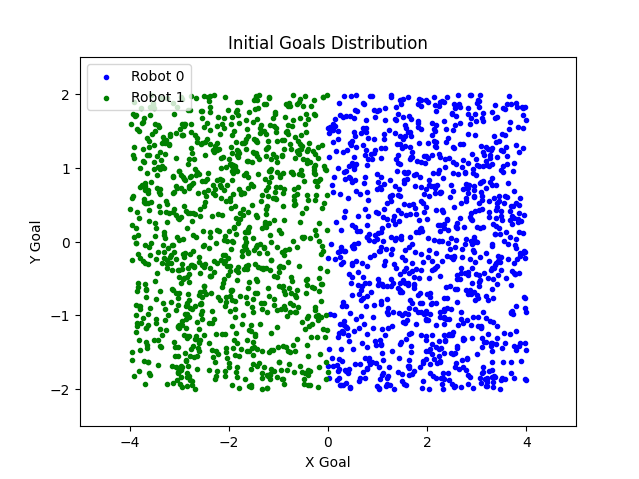
\includegraphics[width=0.4\textwidth]{docs/latex/figures/train_goals_distribution.png}
    \caption{Plot of abs(u2-u3)) as a function of Xij}
\end{figure}

\begin{figure}[h!]
    \centering
    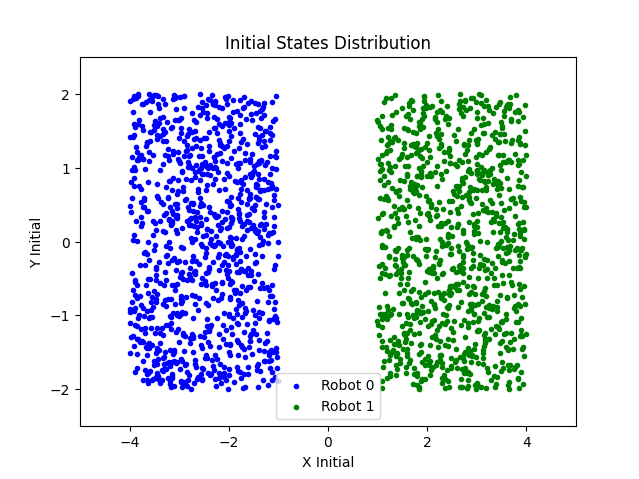
\includegraphics[width=0.4\textwidth]{docs/latex/figures/train_states_distribution.png}
    \caption{Plot of abs(u2-u3)) as a function of Xij}
\end{figure}

\section{Conclusion}
In this paper, we have adapted the method from Chen et. al. \cite{chen2017cadrl}, modifying several parameters and functions. In order to evaluate our method, we compared it to ORCA over 1000 sample trajectories.

\bibliographystyle{IEEEtran.bst}
\bibliography{references.bib}
\end{document}
